The empirical part is divided into blbnalanb

\section{Testing Configuration}
This section delves into the configuration and setup of our empirical testing. We begin by presenting our carefully selected datasets, which serve as the foundation for our evaluation. We highlight specific insights and characteristics of these datasets that make them compelling choices for our study. Afterward, we focus on the models we employ for testing and subsequent result comparison. We provide a comprehensive overview of the selected models, outlining their key features and motivations behind their inclusion in our evaluation. Subsequently, we provide a detailed description of the training pipeline and explain specific hyperparameters for which we will optimize these models.

\subsection{Datasets}
We will first explain our choice of datasets and introduce each dataset individually. Afterward, we will explore essential observations that are to be considered when assessing the actual empirical results.

\subsubsection{Choice of Datasets}
In selecting the datasets for our thesis, we adhered to two fundamental principles to ensure the robustness and diversity of our evaluation for \gnn and \wlnn models. The first principle focuses on using widely recognized benchmark datasets that have been extensively employed in previous studies. This principle enables us and readers to make meaningful comparisons with existing results. The second principle focuses on choosing datasets that are distinct from one another in terms of both their application domains and the way they encode information in graphs.

To fulfill the first principle, we opted for datasets from the TUDataset library. This library, curated by \cite{Mor+2020}, serves as a widely recognized standard for evaluating graph-related methods.

Regarding the second principle, we incorporated the insights from \cite{Liu2022}, who developed a comprehensive taxonomy of common graph benchmark datasets. Their work examined the degree to which information is encoded in graph structures compared to node features with respect to solving the task of the datasets. Based on their taxonomy, they categorized datasets into three distinct classes:
\begin{enumerate}
	\item Datasets in which the most crucial information for solving the task is contained in the node features.
	\item Datasets similar to the first category, but with the significant exception that the node degree strongly correlates with the node features. In these datasets, utilizing simple structural information, such as computing the node degree, is as beneficial for solving the task as using the original node features.
	\item Datasets where the most crucial information is encoded within the graph structure itself.
\end{enumerate}
These categories help us understand how information is encoded in various datasets, such that we aim to choose datasets from all three categories.

As a result of considering these two principles, we selected the following datasets for our thesis: \textsc{Enzymes}, \textsc{Imdb-Binary}, \textsc{Mutag}, \textsc{Nci1}, \textsc{Proteins}, and \textsc{Reddit-Binary} for classification tasks, and \textsc{Alchemy} and \textsc{Zinc} for regression tasks. For an overview of the elemental properties of each dataset, see \cref{tab:overview_datasets}. We will now shortly introduce each dataset individually: \newline

\textsc{Enzymes}, provided by \cite{Borgwardt2005}, is a dataset consisting of proteins in their tertiary structure, categorized into six distinct enzyme classes. Each node represents a secondary structure, and has an edge to its three spatially closest nodes. Furthermore, each node feature encodes the type of secondary structure (\textit{helix}, \textit{sheet} or \textit{turn}), as well as physical and chemical information. \newline


\textsc{Imdb-Binary}, provided by \cite{Yanardag2015}, is a dataset comprising ego networks. Each node in the network represents an actor/actress, and a unidirectional edge exists between two nodes if and only if the corresponding actors played together in a movie. The task involves determining whether each ego network's genre is \textit{action} or \textit{romance}. \newline

\textsc{Mutag}, provided by \cite{Debnath1991}, is a dataset comprising Nitroaromatic compounds. Each compound is represented by a graph in which nodes represent atoms, with their types encoded as node features, and edges represent atomic bonds. The task involves determining whether a given compound has a mutagenic effect on Salmonella typhimurium bacteria. \newline

\textsc{Nci1}, provided by \cite{Wale2008}, comprises graph representations of chemical compounds. In these graphs, nodes represent atoms, and edges represent atomic bonds. Moreover, the atom types are encoded in the node features. The overall task involves determining whether a given compound is active or inactive in inhibiting non-small cell lung cancer.\newline

\textsc{Proteins}, provided by \cite{Borgwardt2005}, contains proteins encoded similarly to ENZYMES. The task here is to determine whether each graph represents an enzyme. \newline

\textsc{Reddit-Binary}, provided by \cite{Yanardag2015}, involves graphs that are derived from popular Reddit communities. The nodes in these graphs represent users who are active in the community, while the edges represent interactions between the users. The task is to identify whether a graph belongs to a community that is focused on questions and answers, or one that is focused on discussions. \newline

\textsc{Alchemy}, provided by \cite{Chen2019alchemy}, consists of organic molecules, with each node representing an atom and each edge representing an atomic bond. Additionally, each node feature encodes various properties for each atom, while each edge encodes the bond type and distance between atoms. The overall task is to compute 12 different continuous quantum mechanical properties for each graph. \newline

\textsc{Zinc}, provided by \cite{Bresson2019} and \cite{Irwin2012}, consists of molecular graphs where each node represents a heavy atom, and the corresponding node feature specifies its type. The edges in the graph encode the bonds between atoms, and their features further describe the type of bond. The task is to calculate a molecular property known as constrained solubility ($\log P - \text{SA} - \text{cycle}$).\newline

\begin{table}[]
	\begin{center}
		\caption{Dataset statistics and properties for graph-level prediction tasks. This table has been adapted from \cite{Morris2022}.}
		\resizebox{0.975\textwidth}{!}{ 	\renewcommand{\arraystretch}{1.05}
			\begin{tabular}{@{}c <{\enspace}@{}lccccccc@{}}\toprule
				& \multirow{3}{*}{\vspace*{4pt}\textbf{Dataset}} & \multicolumn{7}{c}{\textbf{Properties}}\\
				\cmidrule{3-9}
				                         & & \shortstack{Number\\of graphs} & \shortstack{Number of\\classes/targets} & \shortstack{$\varnothing$ Number\\of nodes} & \shortstack{$\varnothing$ Number\\ of edges} & \shortstack{Node\\labels} & \shortstack{Edge\\labels} & \shortstack{Taxonomy \\Category} \\ \midrule
				\multirow{6}{*}{\rotatebox{90}{Classification}}
				& $\textsc{Enzymes}$       & 600               & 6                         & 32.6                          & 62.1                          & \cmark                   & \xmark  & 1    \\
				& $\textsc{IMDB-Binary}$   & 1\,000            & 2                         & 19.8                          & 96.5                          & \xmark                   & \xmark   & 3   \\
				& $\textsc{Mutag}$         & 188               & 2                         & 17.9                          & 19.8                          & \cmark                   & \xmark   & 2   \\
								
				& $\textsc{NCI1}$          & 4\,110            & 2                         & 29.9                          & 32.3                          & \cmark                   & \xmark   & 3   \\
				& $\textsc{Proteins}$      & 1\,113            & 2                         & 39.1                          & 72.8                          & \cmark                   & \xmark  & 2    \\
				& $\textsc{Reddit-Binary}$ & 2\,000            & 2                         & 429.6                         & 497.8                         & \xmark                   & \xmark & 3     \\ 
				\midrule
				\multirow{2}{*}{\rotatebox{90}{Reg.}}
				& $\textsc{Alchemy}$       & 202\,579          & 12                        & 10.1                          & 10.4                         & \cmark                   & \cmark & -     \\
				& $\textsc{Zinc}$       & 249\,456          & 1                        & 23.1                         & 24.9                          & \cmark                   & \cmark & -     \\
				\bottomrule
			\end{tabular}}
		\label{tab:overview_datasets}
	\end{center}
\end{table}

\subsubsection{Analysis of the Datasets}
To ensure the reliability and fairness of our evaluation, one of our initial steps was to assess the balance of our selected datasets for classification. We employed the normalized Shannon index to evaluate the balance of a dataset, where a value close to $0$ indicates maximum imbalance, while a value close to $1$ signifies perfect balance. See \cref{sec:definition_shannon_index} in the Appendix for a formal definition of this metric.

\begin{table}[H]
	\caption{An overview of the normalized Shannon index calculated for each dataset.}
	\label{tab:shannon_index}
	\centering
    \resizebox{.975\textwidth}{!}{ 	\renewcommand{\arraystretch}{0.9}
		\begin{tabular}{@{}c <{\enspace}@{}lcccccc@{}}	\toprule
			& \multirow{3}{*}{\vspace*{4pt}}&\multicolumn{6}{c}{\textbf{Dataset}}\\\cmidrule{3-8}
			& & {\textsc{Enzymes}}          & {\textsc{Imdb-Multi}}  & {\textsc{Mutag}}           & {\textsc{NCI1}}       & {\textsc{Proteins}}  & {\textsc{Reddit-Binary}}
			\\
			\toprule
			\multirow{1}{*}{} 	&
			Shannon index & 1 & 1 & 0.920 & 1 & 0.973 & 1 \\
			\bottomrule
		\end{tabular}}              
\end{table}

\Cref{tab:shannon_index} provides an overview of the normalized Shannon index computed for each selected classification dataset. Upon analyzing the data, we observed that all the datasets exhibit high balance, as all their values are close to $1$. This finding assures us that the datasets do not suffer significant class imbalances, which will remain important in the following section.

In addition to the balance of all datasets, another important aspect is understanding the upper bound of performance achievable by both \gnn and \wlnn models on these datasets. Unlike in other areas of machine learning where multilayer perceptron models can achieve near-perfect performance due to their universal approximation capabilities (\cite{Hornik1991}), \gnn and \wlnn models have inherent limitations on their expressiveness. This restriction stems from the fact that the expressiveness of the \wl algorithm limits the performance of both frameworks. In detail, if the \wl algorithm can not distinguish a pair of graphs in a dataset, then neither a \gnn nor a \wlnn model can.

While we have pointed out that the \wl algorithm is, in general, quite powerful in distinguishing pairs of graphs in \cref{sec:related_work}; we also explained that it is not complete. Therefore, assuming that \gnn or \wlnn models exist that can achieve almost perfect accuracy on all classification datasets is not reasonable. Thus, we calculated the theoretical maximum accuracy achievable by the perfect model for each dataset. In detail, we even investigated how many iterations of the \wl algorithm it takes to achieve this accuracy. For a comprehensive overview of the accuracies achievable on all datasets, please refer to \cref{tab:max_accuracies}. In this table, we have included the accuracy achievable when running the \wl algorithm for $0$ iterations, which essentially means taking the initial node features as the coloring for iteration $0$ and assessing the expressiveness of this initial coloring.

\begin{table}[H]
	\caption{An overview of the maximum theoretical classification accuracy achievable for each dataset based on the number of \wl iterations in percent. A hyphen ``-'' indicates that the maximum accuracy has converged with fewer iterations, implying that further iterations do not improve the accuracy.}
	\label{tab:max_accuracies}
    \resizebox{.975\textwidth}{!}{ 	\renewcommand{\arraystretch}{0.9}
		\begin{tabular}{@{}c <{\enspace}@{}lcccccc@{}}	\toprule
			& \multirow{3}{*}{\vspace*{4pt}\textbf{1-WL}}&\multicolumn{6}{c}{\textbf{Dataset}}\\\cmidrule{3-8}
			& & {\textsc{Enzymes}}         &  {\textsc{Imdb-Binary}}  & {\textsc{Mutag}}           & {\textsc{NCI1}}       & {\textsc{Proteins}}  & {\textsc{Reddit-Binary}}
			\\
			\toprule
			\multirow{6}{*}{} 	&
			Iterations: $0$       &  81.4 & 60.6 & 93.1 & 91.3 & 91.9 & 83.9
			\\ 
			& Iterations: $1$    & 100.0 & 88.6 & 95.7 & 99.5 & 99.7 & 100.0
			\\
			& Iterations: $2$    & - & - & 99.5 & 99.8 & - & - 
			\\
			& Iterations: $3$   & - & - & 100.0 & 99.8 & - & - 
			\\
			& Iterations: $4$    & - & - & - & - & - & -
			\\
			\cmidrule{2-8}\morecmidrules\cmidrule{2-8}
			& Max Accuracy     & 100.0 & 88.6 & 100.0 & 99.8 & 99.7 & 100.0      
			\\
			\bottomrule
		\end{tabular}}              
\end{table}

Upon examining the results, we observe that all datasets exhibit perfect or near-perfect theoretical classification accuracies. This result makes interpreting results obtained from actual \wlnn or \gnn models later on more straightforward. Additionally, the accuracy achievable after each number of iterations provides a theoretical lower limit on the number of message-passing layers a \gnn must be composed of to be even capable of achieving this accuracy. 

We have conducted the same analyzes on additional datasets, as their results might be valuable to the reader. For these, see \cref{tab:max_accuracies_app} in the Appendix.


\subsection{Choice of Models}
In selecting our models, we aimed to use techniques that are relatively generic and not highly specialized for any of the datasets, such that insights we gain upon analyzing the model's performance can be generalized better. Consequently, we opted for a basic set of models to maintain simplicity and versatility.

\subsubsection{\wlnn Models}
Our primary consideration for the \wlnn models revolves around choosing an encoding function, as all other components are fixed. To keep things straightforward, we decided to employ encoding functions consisting of two main components. Firstly, an optional preprocessing step that operates on the colors computed by the \wl algorithm. Secondly, a basic pooling function for transforming the color histogram into a fixed-size vector.

In more detail, the optional preprocessing step involves a simple look-up table. If utilized, this step maps each color injectively to a vector in the range of $[-1, 1]^n$, where the value of $n$ is a hyperparameter. By encoding the color information into higher dimensions, this approach aims to enhance efficiency during subsequent processing steps. For the second step, the pooling component, we selected elementary functions such as elementwise \textsf{Max}, \textsf{Mean}, and Summation (\textsf{Sum}). In summary, each of the \wlnn models can be uniquely identified by their encoding functions; therefore, we will refer to each model by their encoding function as follows:
\begin{equation*}
	\text{Embedding}-\{\textsf{Max}, \textsf{Mean}, \textsf{Sum}\} \quad \text{or} \quad \{\textsf{Max}, \textsf{Mean}, \textsf{Sum}\},
\end{equation*}
where ``Embedding'' indicates the use of the optional preprocessing step.

\subsubsection{\gnn Models}
As mentioned in the introduction to this section, our focus is on keeping the models basic. Hence, we opted for \gin by \cite{Xu2018}, \gcn by \cite{Kip+2017}, and \gat by \cite{Velivckovic2017} as the base architecture for the message-passing layers. Each of these architectures was chosen for specific reasons.

Firstly, we included \gin as an obvious candidate because it has been proven to be as expressive as the 1-WL algorithm. This characteristic makes it interesting when comparing it to \wlnn models.
Next, we also included \gcn based on its good empirical success in recent years. Furthermore, the insights provided by \cite{Nikolentzos2023} demonstrated that, in a certain sense, the node features computed by \gcn and \gin are similar, making \gcn a reasonable alternative to \gin in cases where the advantage of \gin's expressiveness is not needed.
Lastly, we added \gat as an alternative approach to the other two architectures. In detail, \cite{Nikolentzos2023} also showed that the node features computed by \gat are entirely different from those computed by \gin or \gcn.

Regarding the choice of \textsf{Readout} functions, we decided to utilize functions that are composed of two components. The first component is one of the elementwise pooling functions, such as \textsf{Max}, \textsf{Mean}, and \textsf{Sum}, to aggregate the information from a graph representation into a fixed-sized vector. Secondly, we incorporate a multilayer perceptron to process the aggregated information further, similarly to the \wlnn models.

In summary, each of the \gnn models can be uniquely identified by their \gnn architecture and the pooling function utilized; therefore, we will refer to each model by these two properties as follows:
\begin{equation*}
	{\{\gat, \gcn, \gin\}} - \{\textsf{Max}, \textsf{Mean}, \textsf{Sum}\}.
\end{equation*}

Note that the selection of the Readout function creates similarities between the \gnn and \wlnn models. These similarities play a crucial role in ensuring that any empirical differences observed between the two frameworks are not attributed to the utilization of more powerful techniques.

\subsection{Experimental Setup}

For the empirical testing, we took measures to ensure the reliability of our results in terms of hyperparameter configuration. Additionally, we aimed to ensure the reproducibility of the training pipeline for each model.

\subsubsection{Testing Procedure}

We started by conducting tests on the classification datasets, which serve as the basis for our evaluation. In our testing code, we employ a 10-fold cross-validation approach. Within this framework, we further partitioned the training data randomly, allocating 10\% of it for validation purposes. Consequently, each training iteration consisted of 0.81\% of the original dataset as the training set, 9\% as the validation set, and 10\% as the test set. We repeat this testing procedure five times to mitigate the influence of randomness on the model's performance. Ultimately, we recorded the mean accuracy on the test set along with its standard deviation as the primary performance metric of the model. Note that the use of standard cross-validation for generating the splits and the choice of mean accuracy as our primary metric is reasonable and justified as the datasets are highly balanced, as demonstrated in Section 2.

In the case of the regression datasets, we adopted a slightly different testing procedure. Due to their larger scale compared to the classification datasets, we opted for a more time-efficient approach. To achieve this, we utilized pre-existing training pipelines developed in \cite{Mor+2020} and \cite{Morris2022speqnets}. These pipelines use a fixed training, validation, and test split, accelerating the testing process. Similar to the classification datasets, we performed five runs for each model configuration and conducted a hyperparameter sweep for all model configurations. We record the mean absolute error and its standard deviation, as well as the mean logarithmic absolute error and its standard deviation across all runs. Furthermore, we test two splits for each regression dataset: one utilizing only 10,000 samples for training, while the other split uses the entire training set.

\subsubsection{Hyperparameter Optimization}\cref{sec:hyperparam}
To ensure the comparability of our results with other works and limit the number of hyperparameters requiring optimization, we followed standard practices when configuring our models. Detailed information on all hyperparameters, including the ones we optimized, can be found in \cref{tab:sweep_wlnn} for the \wlnn models used in classification tasks, \cref{tab:sweep_gnn} for the \gnn models employed in classification tasks, and \cref{tab:sweep_wlnn_reg} for the \wlnn models utilized in the regression task in the Appendix. We will shortly discuss the most critical parameters we optimized for:

Early in our investigations, we made a significant observation regarding the learning performance of \wlnn models. We noticed considerable performance discrepancies when comparing \wlnn models using the standard version of the \wl algorithm with the one from GNNs. Consequently, we investigated the possibility of parametrizing the \wl algorithm to enhance control over the expressiveness of the colorings it computes. Specifically, we focused on two crucial parameters: 1) the number of iterations and 2) the usage of its convergence behavior as an early termination criterion.

The advantage of this more granular parametrization is that it enables us to apply the same number of \wl iterations to each graph processed by a \wlnn model by deactivating the convergence behavior and fixing the number of iterations. By deactivating this behavior and keeping the number of iterations minimal, we observed that the number of colors used by the \wl algorithm remained contained. As a result, the \mlp component of each \wlnn model seems to generalize better, significantly improving performance. Therefore, one of the most crucial hyperparameters we optimized for all \wlnn models was the number of \wl iterations. Additionally, if employed, the size of the dimension of the look-up table was another significant parameter to optimize.

In contrast, the hyperparameter selection for the \gnn models was relatively less intricate. The key parameters of interest here are the number of message-passing layers and the size of the hidden dimensions used in each layer. The reason for this is that the number of layers directly corresponds to the expressiveness of the GNN, as demonstrated in the proof, while the size of the hidden dimensions enables easier learning by allowing the model to store more information during graph processing.

\subsubsection{Implementation Details and Result Accessibility}
The implementation of our models and training procedures was carried out using \textsc{Python 3.10} along with the open-source library \textsc{PyTorch}\footnote{Open source machine learning framework that was originally developed by Meta AI and does now belong to the Linux Foundation umbrella. \href{https://pytorch.org}{https://pytorch.org}} and its extension \textsc{PyTorch Geometric}\footnote{Open source library that acts as an extension to PyTorch and allows for easy writing and training of graph neural networks. \href{https://pytorch-geometric.readthedocs.io/en/latest}{https://pytorch-geometric.readthedocs.io}}. Moreover, we leveraged \textsc{Weights\&Biases} as our tool for coordinating and recording the results of the hyperparameter sweeps. The code for our experiments is publicly available on \textsc{GitHub} at \url{https://github.com/ericbill21/BachelorThesis}, and the corresponding results can be accessed via \textsc{Weights\&Biases} at \url{https://wandb.ai/eric-bill/BachelorThesisExperiments}. We conducted our tests on the RWTH High Performance Computing cluster by the RWTH Aachen University as well as on private hardware.

\section{Empirical Testing}
In this section we present our empirical findings. See Table 3 for an overview of the performance metric achieved by the best performing configuration of each model on each dataset. Furthermore, see Table 4 for a similiar overview for the regression datasets.

\begin{table}[H]
	\caption{Overview of the classification accuracies achieved by the best model of each configuration for each dataset in percent and standard deviation.}
	\label{tab:my_label}
    \resizebox{.975\textwidth}{!}{ 	\renewcommand{\arraystretch}{1.05}
		\begin{tabular}{@{}c <{\enspace}@{}lcccccc@{}}	\toprule
			& \multirow{3}{*}{\vspace*{4pt}\textbf{Method}}&\multicolumn{6}{c}{\textbf{Dataset}}\\\cmidrule{3-8}
			& & {\textsc{Enzymes}}         &  {\textsc{Imdb-Binary}}      & {\textsc{Mutag}}           & {\textsc{NCI1}}       & {\textsc{Proteins}}           & 
			{\textsc{Reddit-Binary}}
			\\
			\toprule
			\multirow{6}{*}{\rotatebox{90}{$\wlnn$}} 	&
			\textsf{Max} & 16.7 \scriptsize $\pm 4.2$ & 52.0 \scriptsize $\pm 5.3$	&73.8 \scriptsize $\pm 12.4$ &	58.6 \scriptsize $\pm 3.3$ & 62.9 \scriptsize $\pm 4.9$  & 	69.2 \scriptsize $\pm 4.0$
			\\ 
			& \textsf{Mean} & 18.2 \scriptsize $\pm 4.8$  &	59.4 \scriptsize $\pm 5.8$ &	77.1 \scriptsize $\pm 11.5$	 & 64.0 \scriptsize $\pm 3.3$ &	60.9 \scriptsize $\pm 4.5$ & 66.1 \scriptsize $\pm 3.2$   
			\\ 	
			& \textsf{Sum} & 18.0 \scriptsize $\pm 6.2$	 & 57.5 \scriptsize $\pm 5.1$ & 66.8 \scriptsize $\pm 13.9$ & 56.9 \scriptsize $\pm 3.8$ & 65.6 \scriptsize $\pm 4.8$ & 73.0 \scriptsize $\pm 5.1$   
			\\  
			\cmidrule{2-8}  		
			& \textsf{Embedding-Max} & 40.5  \scriptsize	$\pm 7.4$         & 69.4  \scriptsize $\pm 4.9$             & 81.1 \scriptsize $\pm 11.2$	 & 82.7  \scriptsize $\pm 2.0$          & \textbf{75.2} \scriptsize $\pm 3.9$ & 0.0 \scriptsize $\pm 0.0$        
			\\ 
			& \textsf{Embedding-Mean}     & 42.6 \scriptsize	$\pm 9.0$ & \textbf{72.4}     \scriptsize $\pm 4.1 $         & 84.1 \scriptsize $\pm 9.1$	       & 83.1   \scriptsize $\pm 1.9$         & 72.3  \scriptsize $\pm 4.2$         &  0.0 \scriptsize $\pm 0.0$                     
			\\ 
			& \textsf{Embedding-Sum} & \textbf{48.3} \scriptsize	$\pm 8.1$          & 72.0  \scriptsize $\pm 3.8$             & \textbf{85.1} \scriptsize $\pm 8.6$	     & \textbf{83.6}   \scriptsize $\pm 2.2$         & 75.2  \scriptsize $\pm 4.5$   	& 0.0  \scriptsize $\pm 0.0$                     
			\\ 
			\cmidrule{2-8}
			\multirow{9}{*}{\rotatebox{90}{Graph Neural Networks}} 
			& \textsf{GAT:Max}                    & 31.2 \scriptsize $\pm 6.0$        & 70.7 \scriptsize $\pm 4.8$          & 71.1 \scriptsize $\pm 12.2$ & 58.0 \scriptsize $\pm 4.2$          & 72.5 \scriptsize $\pm 5.1$         & 0.0 \scriptsize $\pm 0.0$  
			\\ 
			& \textsf{GAT:Mean}    & 28.9 \scriptsize $\pm 5.9$          & 70.9 \scriptsize $\pm 3.7$           & 74.8 \scriptsize $\pm 9.1$            & 66.1 \scriptsize $\pm 2.8$         & 64.9 \scriptsize $\pm 6.4$       & 0.0 \scriptsize $\pm 0.0$
			\\ 
			& \textsf{GAT:Sum}                  & \textbf{34.4} \scriptsize $\pm 7.0$          & 72.2 \scriptsize $\pm 4.5$	            & 82.1 \scriptsize $\pm 11.2$            & 69.8 \scriptsize $\pm 2.6$	          & 73.4 \scriptsize $\pm 3.9$
			& 0.0 \scriptsize $\pm 0.0$          
			\\
			
			\cmidrule{2-8}
					
			& \textsf{GCN:Max} & 33.1 \scriptsize $\pm 7.5$ &	73.5 \scriptsize $\pm 4.1$	& 74.5 \scriptsize $\pm 11.3$ & 61.1 \scriptsize $\pm 3.6$ &	69.8 \scriptsize $\pm 5.9$ & 0.0 \scriptsize $\pm 0.0$  
			\\ 
			& \textsf{GCN:Mean} & 29.9 \scriptsize $\pm 5.7$ &	\textbf{74.7} \scriptsize $\pm 3.8$ & 75.0 \scriptsize $\pm 10.4$ &	68.9 \scriptsize $\pm 2.4$ &	70.9 \scriptsize $\pm 5.2$ & 0.0 \scriptsize $\pm 0.0$
			\\ 
			& \textsf{GCN:Sum} & 31.7 \scriptsize $\pm 7.2$ &	73.0 \scriptsize $\pm 4.4$	& 81.5 \scriptsize $\pm 10.3$ & 70.4 \scriptsize $\pm 2.1$ & 3.5 \scriptsize $\pm 3.9$ & 0.0 \scriptsize $\pm 0.0$                        
			\\
			\cmidrule{2-8}	
						
			& \textsf{GIN:Max} & 29.2 \scriptsize $\pm 6.2$	& 70.8 \scriptsize $\pm 4.7$ & 77.3 \scriptsize $\pm 10.7$ & \textbf{79.9} \scriptsize $\pm 2.2$ & \textbf{74.3} \scriptsize $\pm 5.1$ & 0.0 \scriptsize $\pm 0.0$   
			\\ 
			& \textsf{GIN:Mean}  & 31.7 \scriptsize $\pm 6.7$	& 71.1 \scriptsize $\pm 5.4$ & 82.4 \scriptsize $\pm 9.8$ & 	70.8 \scriptsize $\pm 2.2$ & 72.0 \scriptsize $\pm 4.0$ & 0.0 \scriptsize $\pm 0.0$
			\\ 
			& \textsf{GIN:Sum} & 28.9 \scriptsize $\pm 8.7$ & 	69.5 \scriptsize $\pm 4.8$	& \textbf{84.6} \scriptsize $\pm 8.7$ & 70.8 \scriptsize $\pm 2.3$ &	73.2 \scriptsize $\pm 4.3$ & 0.0 \scriptsize $\pm 0.0$
			\\
			\bottomrule
		\end{tabular}}            
\end{table}

\begin{table}[H]
	\resizebox{0.975\textwidth}{!}{ 	\renewcommand{\arraystretch}{1.05}
	\newcommand{\seq}[2]{$(#1, #2)$\text{-}\textsf{SpeqNet}\xspace}
		\begin{tabular}{@{}lcccc@{}}	\toprule
			\multirow{3}{*}{\vspace*{4pt}\textbf{Method}}&\multicolumn{4}{c}{\textbf{Dataset}}
			\\
			\cmidrule{2-5} 
			& {\textsc{Alchemy}} & {\textsc{Alchemy (10k)}} & {\textsc{Zinc}} & {\textsc{Zinc (10k)}} 
			\\	
			\toprule
			\textsf{GINE-$\varepsilon$}\xspace & 0.103 {\scriptsize $\pm  0.001$} -2.956 {\scriptsize $\pm  0.029$}$^1$ & 0.180 {\scriptsize $\pm  0.006$} -1.958  {\scriptsize $\pm  0.047$}$^2$ & - & 0.084 {\scriptsize $\pm  0.004$}$^1$
			\\
			\midrule
			\textsf{Embedding-Max} & 0.648 {\scriptsize $\pm 0.003$} -0.511 {\scriptsize $\pm 0.009$} &	0.409 {\scriptsize $\pm 0.003$} -1.023 {\scriptsize $\pm 0.009$} &	0.382 {\scriptsize $\pm 0.005$} &	0.659 {\scriptsize $\pm 0.007$}
			\\
			\textsf{Embedding-Mean} & 0.617 {\scriptsize $\pm 0.003$} -0.564 {\scriptsize $\pm 0.005$} &	0.355 {\scriptsize $\pm 0.004$} -1.269 {\scriptsize $\pm 0.020$} &	\textbf{0.348} {\scriptsize $\pm 0.010$} &	0.484 {\scriptsize $\pm 0.009$}
			\\
			\textsf{Embedding-Sum} & \textbf{0.600} {\scriptsize $\pm 0.004$} -0.625 {\scriptsize $\pm 0.032$} & \textbf{0.305} {\scriptsize $\pm 0.001$} -1.740 {\scriptsize $\pm 0.042$} &	0.384 {\scriptsize $\pm 0.004$} &	\textbf{0.465} {\scriptsize $\pm 0.009$}
			\\
			\bottomrule
	\end{tabular}}
	\caption{Mean MAE (mean std.\ MAE, logMAE) on large-scale (multi-target) molecular regression tasks. The results marked by $^1$ are adopted from \cite{Mor+2020} and by $^2$ from \cite{Morris2022}.}
\end{table}

As an eraly interpretation one can see that the best \wlnn models are capable of achieving the a very similiar performance in comparison to \gnn (e.g. IMDB) or even better in all other case a better performance, with some examples having a huge difference compared to the \gnn model. But only on the classification datasets. In the regression datasets, we see that all \wlnn models perform quite poorly compared to the \gnn model. Also interesting is the differnece we record between the two regression datasets. While there is a signifcant performance difference between the using the entire dataset or just a subset for the dataset Alchemy, this difference seems not to exist for Zinc.

In the following sections we will build up on these results an provide furhter insights and analyses into \wlnn and \gnn models.

\subsection{WL too expressive?}
As already outlined in \cref{sec:hyperparam} we investigated early on to limit the expressiveness the \wl alogorithm offers by trying to contain the number of colors this alogrithm uses. In particular we allowed to fix the number of iterations of the \wl alogrithm in a \wlnn model. The idea was that every graph processed by such a model, would be than mapped to a coloring which is in a similar color range as all the other graphs. Thereby limiting the total number of colors, such that no oultier cases are created. 

If we compare the results of \wlnn models utilizing the standard \wl alogorithm compared to the parametrized version of our see a signifcant difference in performance accross all classification datasets. See Table 5, for an overview of the best accuracy achieved by these models in comparison to our parametrized models. The data confirms our believes, that the \wl alogirhtm is for some task to expressive, as there is a signifcant performance difference between the two types.

\begin{table}[H]
    \resizebox{.975\textwidth}{!}{ 	\renewcommand{\arraystretch}{1.05}
		\begin{tabular}{@{}c <{\enspace}@{}lcccccc@{}}	\toprule
			& \multirow{2}{*}{\vspace*{4pt}\textbf{Property}}&\multicolumn{6}{c}{\textbf{Dataset}}\\\cmidrule{3-8}
			& & {\textsc{Enzymes}}         &  {\textsc{Imdb-Binary}}      & {\textsc{Mutag}}           & {\textsc{NCI1}}       & {\textsc{Proteins}}           & 
			{\textsc{Reddit-Binary}}
			\\
			\toprule
			\multirow{1}{*}{}
			& Standard \wl & 34.2 \scriptsize $\pm 6.7$	& 67.0 \scriptsize $\pm 4.3$ & 76.3 \scriptsize $\pm 9.4$ & & 71.4 \scriptsize $\pm 4.9$ & 70.9 \scriptsize $\pm 3.8$
			\\
			& Parametrized \wl & 48.3 \scriptsize $\pm 8.1$	& 72.4 \scriptsize $\pm 4.1$ & 85.1 \scriptsize $\pm 8.6$ & 83.6 \scriptsize $\pm 2.2$ & 75.2 \scriptsize $\pm 3.9$	& 78.4 \scriptsize $\pm 2.7$
			\\
			\bottomrule
		\end{tabular}}
		\caption{Comparison between the best performing \wlnn models using the standard \wl algorithm and the one employing the parametrized version of it in percent.}
        \label{tab:my_label4}     
\end{table}

Following the insights, another interesting observation is than to investigate which number of \wl iteration in particular leads to the best performing models. To put this into perspective, we created Figure 2 where over all models we tested, we plotted for each the performance achieved grouped by the number of iterations. 

\begin{figure}
	\centering
	\begin{subfigure}[b]{0.19\textwidth}
		\centering
		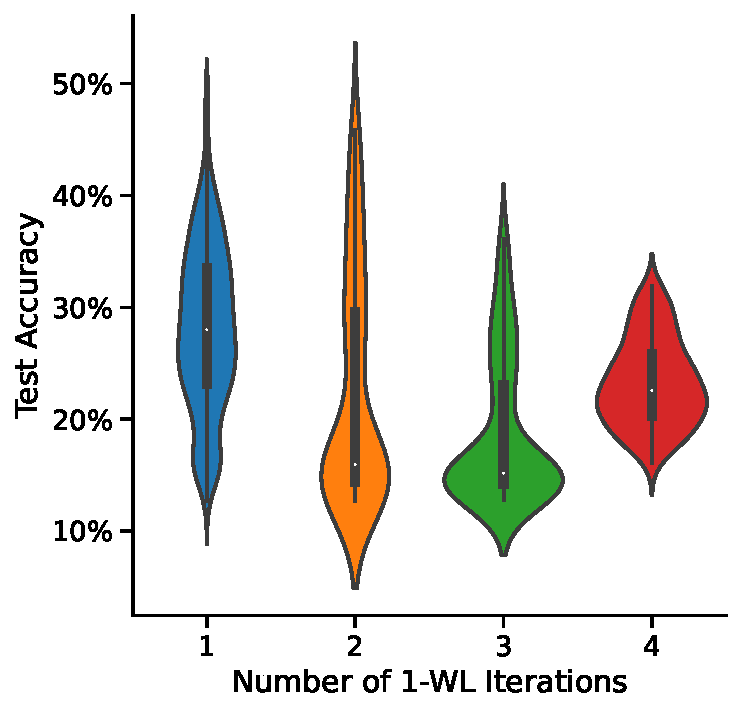
\includegraphics[width=\textwidth]{Figures/k_wl_violin_ENZYMES.pdf}
        \caption{\scriptsize\textsc{Enzymes}}
	\end{subfigure}
	\hfill
	\begin{subfigure}[b]{0.19\textwidth}
		\centering
		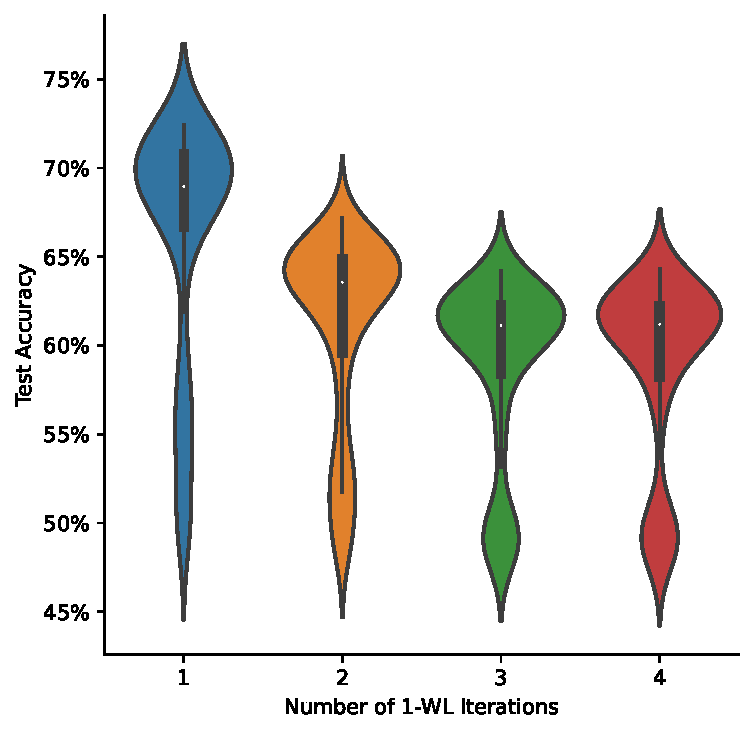
\includegraphics[width=\textwidth]{Figures/k_wl_violin_IMDB-BINARY.pdf}
        \caption{\scriptsize\textsc{Imdb-Binary}}
	\end{subfigure}
	\hfill
	\begin{subfigure}[b]{0.19\textwidth}
		\centering
		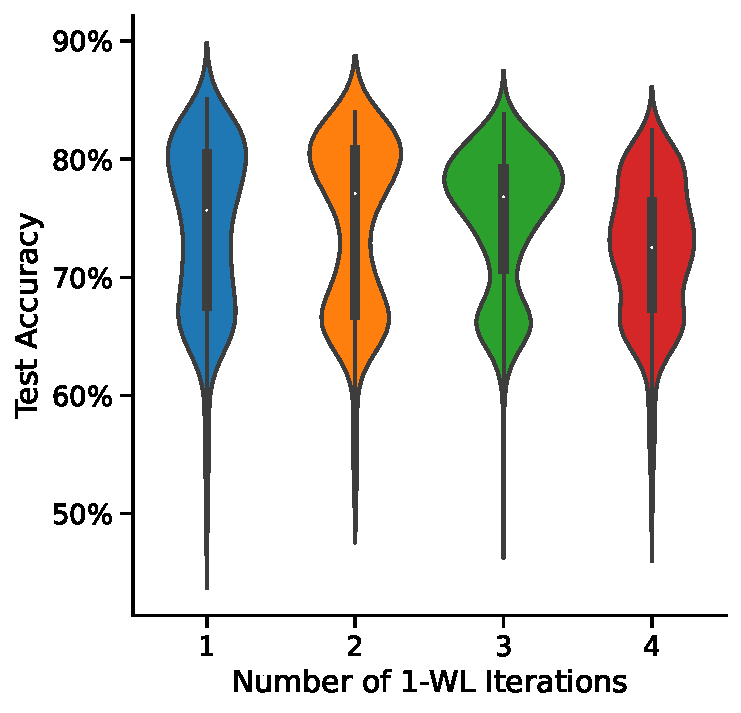
\includegraphics[width=\textwidth]{Figures/k_wl_violin_MUTAG.pdf}
        \caption{\scriptsize\textsc{Mutag}}
	\end{subfigure}
	\hfill
	\begin{subfigure}[b]{0.19\textwidth}
		\centering
		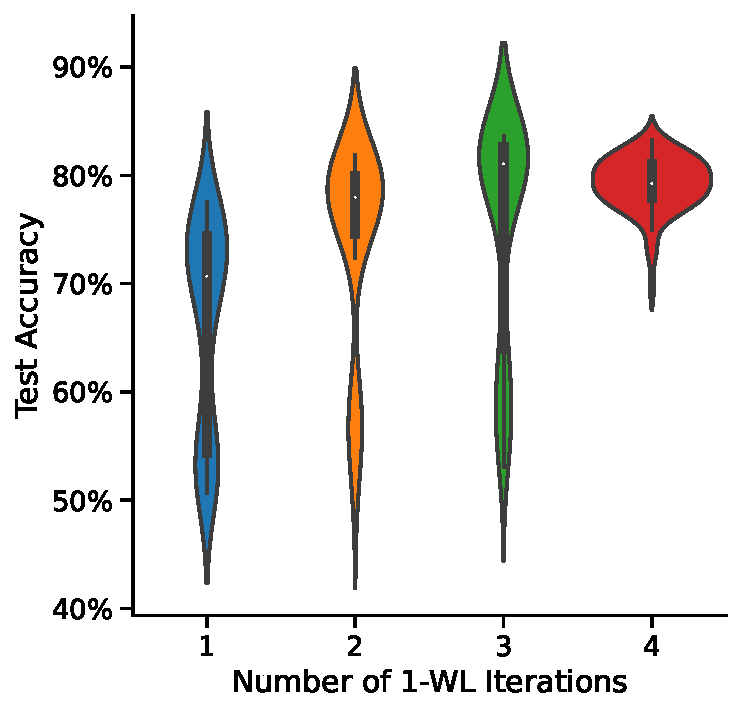
\includegraphics[width=\textwidth]{Figures/k_wl_violin_NCI1.pdf}
        \caption{\scriptsize\textsc{Nci1}}
	\end{subfigure}
	\hfill
	\begin{subfigure}[b]{0.19\textwidth}
		\centering
		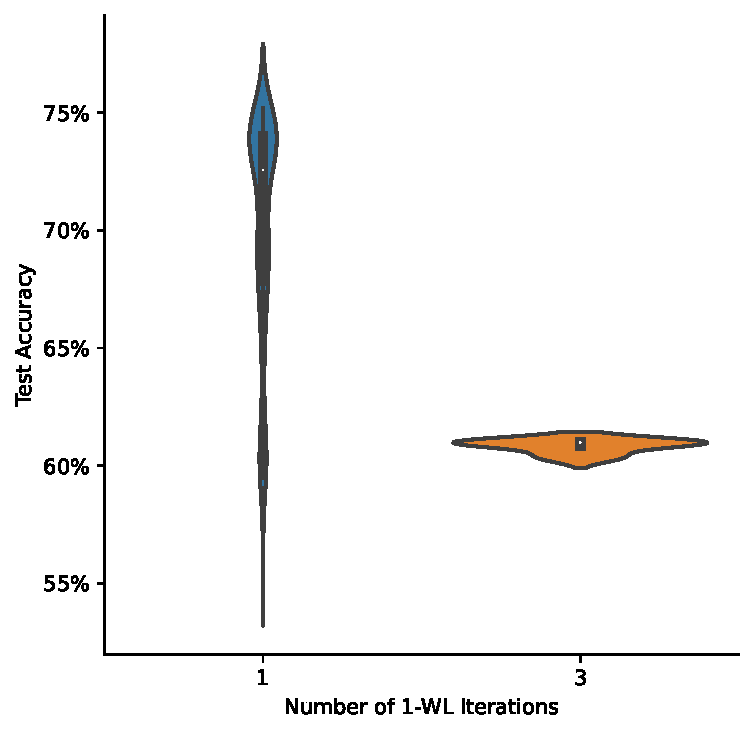
\includegraphics[width=\textwidth]{Figures/k_wl_violin_PROTEINS.pdf}
        \caption{\scriptsize\textsc{Proteins}}
	\end{subfigure}
	\par\bigskip
	\begin{subfigure}[b]{0.19\textwidth}
		\centering
		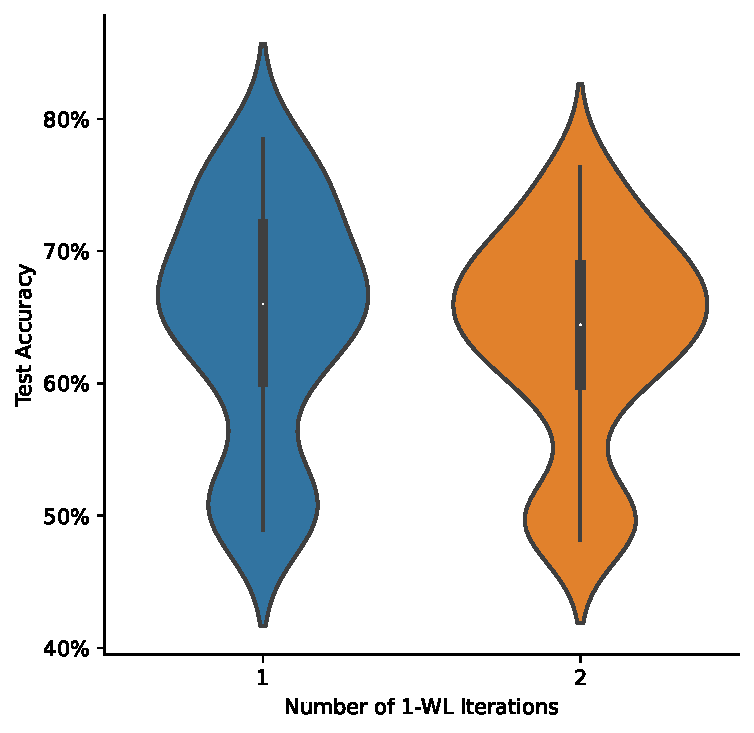
\includegraphics[width=\textwidth]{Figures/k_wl_violin_REDDIT-BINARY.pdf}
        \caption{\scriptsize \textsc{Reddit-Binary}}
	\end{subfigure}
	\hfill
	\begin{subfigure}[b]{0.19\textwidth}
		\centering
		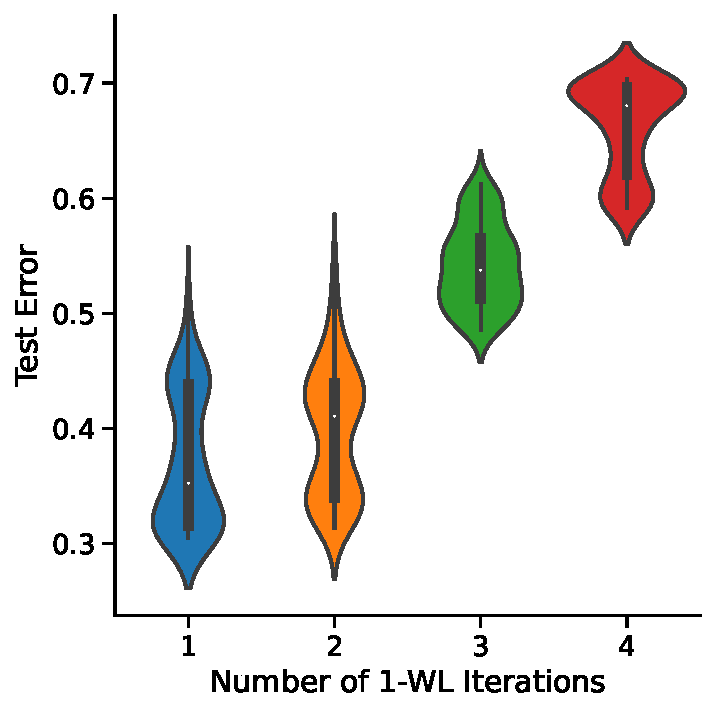
\includegraphics[width=\textwidth]{Figures/k_wl_violin_Alchemy10K.pdf}
        \caption{\scriptsize\textsc{Alchemy (10k)}}
	\end{subfigure}
	\hfill
	\begin{subfigure}[b]{0.19\textwidth}
		\centering
		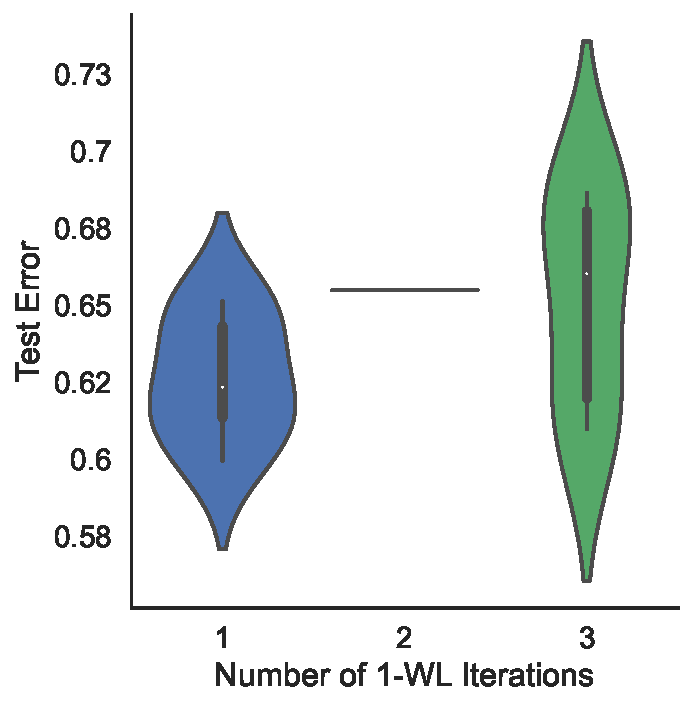
\includegraphics[width=\textwidth]{Figures/k_wl_violin_Alchemy.pdf}
        \caption{\scriptsize\textsc{Alchemy}}
	\end{subfigure}
	\hfill
	\begin{subfigure}[b]{0.19\textwidth}
		\centering
		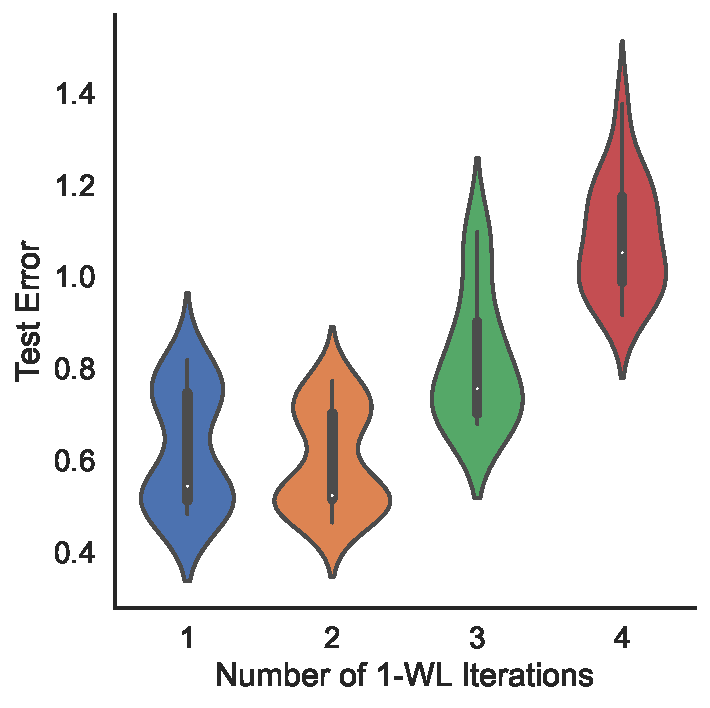
\includegraphics[width=\textwidth]{Figures/k_wl_violin_Zinc 10k.pdf}
        \caption{\scriptsize\textsc{Zinc (10k)}}
	\end{subfigure}
	\hfill
	\begin{subfigure}[b]{0.19\textwidth}
		\centering
		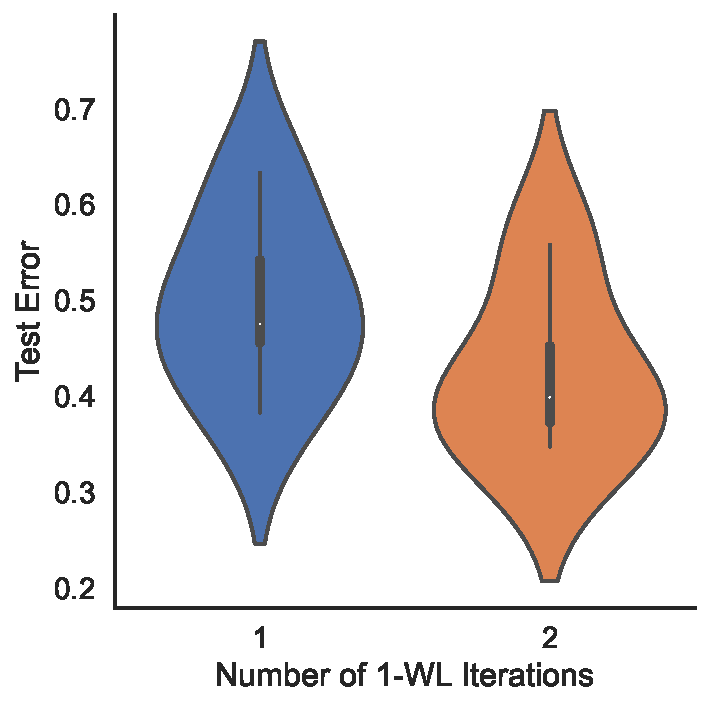
\includegraphics[width=\textwidth]{Figures/k_wl_violin_Zinc.pdf}
        \caption{\scriptsize\textsc{Zinc}}
	\end{subfigure}
	\caption{k\_wl dependence}
	\label{fig:k_wl_dependence}
\end{figure}


\subsection{Explain how results look like}

\section{Discusssion}
\subsection{Learned Lessons}
\subsection{Future Work}

\section{Conclusion}

\newpage


\begin{table}[H]
    \resizebox{.975\textwidth}{!}{ 	\renewcommand{\arraystretch}{1.05}
		\begin{tabular}{@{}c <{\enspace}@{}lcccccc@{}}	\toprule
			& \multirow{3}{*}{\vspace*{4pt}\textbf{Method}}&\multicolumn{6}{c}{\textbf{Dataset}}\\\cmidrule{3-8}
			& & {\textsc{Enzymes}}         &  {\textsc{Imdb-Binary}}      & {\textsc{Mutag}}           & {\textsc{NCI1}}       & {\textsc{Proteins}}           & 
			{\textsc{Reddit-Binary}}
			\\
			\toprule
			\multirow{4}{*}{\rotatebox{90}{$\wlnn$}}
			& \textsf{MLP} & 48.3 \scriptsize	$\pm 8.1$ & \textbf{72.4} \scriptsize	$\pm 4.1$ & 85.1 \scriptsize $\pm 8.6$ & 83.6 \scriptsize	$\pm 4.1$ & \textbf{75.2} \scriptsize $\pm 3.9$
			\\
			& \textsf{SVM Linear} & 34.4 \scriptsize	$\pm 5.5$ & 71.2 \scriptsize	$\pm 3.9$ & 86.4 \scriptsize $\pm 8.9$	 & 83.4 \scriptsize	$\pm 2.1$ & 73.9 \scriptsize $\pm 4.1$
			\\
			& \textsf{SVM RBF} & 45.0 \scriptsize	$\pm 7.0$ & 72.8 \scriptsize	$\pm 4.3$ & 83.2 \scriptsize $\pm 7.5$ & 83.6 \scriptsize	$\pm 1.9$ & 75.2 \scriptsize $\pm 4.0$
			\\
			& \textsf{k-NN} &  \textbf{56.3} \scriptsize $\pm 5.8$ (k=1) & 72.3 \scriptsize $\pm 4.1$ (k=11)& \textbf{86.7} \scriptsize $\pm 7.7$ (k=10) & \textbf{83.9} \scriptsize $\pm 1.8$ (k=5)& 73.9 \scriptsize $\pm 4.1$ (k=19) &
			\\
			\cmidrule{2-8}
			\multirow{4}{*}{\rotatebox{90}{\gnn}}
			& \textsf{MLP} & 34.4 \scriptsize $\pm 7.0$ &  \textbf{74.7} \scriptsize $\pm 3.8$ & 84.6 \scriptsize $\pm 8.7$	 & \textbf{79.9} \scriptsize $\pm 2.2$ & 74.3 \scriptsize $\pm 5.1$
			\\
			& \textsf{SVM Linear} & 33.2 \scriptsize $\pm 5.9$ & 73.9 \scriptsize $\pm 4.2$ & 51.9 \scriptsize $\pm 34.1$ & 67.4 \scriptsize $\pm 2.2$ & 74.7 \scriptsize $\pm 4.2$
			\\
			& \textsf{SVM RBF} & 35.9 \scriptsize $\pm 6.0$ & 74.1 \scriptsize $\pm 3.9$ & \textbf{86.0} \scriptsize $\pm 7.4$ & 73.0 \scriptsize $\pm 1.9$ & 74.6 \scriptsize $\pm 4.6$
			\\ 
			& \textsf{k-NN} & \textbf{51.6} \scriptsize $\pm 7.0$ (k=1)	& 74.3 \scriptsize $\pm 4.0$ (k=132) & 88.3 \scriptsize $\pm 6.5$ (k=38) & 77.5 \scriptsize $\pm 1.7$	(k=2)& \textbf{74.9} \scriptsize $\pm 4.3$ (k=27)&
			\\
			\bottomrule
		\end{tabular}}
		\caption{Overview of the classification accuracies achieved by the best model for each dataset in percent and standard deviation. Additionally, the performance of each model was evaluated under alternative configurations, namely the substitution of the Multilayer Perceptron (MLP) with a Support Vector Machine employing either a linear kernel (SVM Linear) or the Radial Basis Function (SVM RBF), as well as the k-nearest neighbors algorithm (k-NN) with different values for $k$.}
        \label{tab:my_label3}                  
\end{table}

\begin{figure}[H]
	\begin{subfigure}[b]{0.3\textwidth}
		\centering
		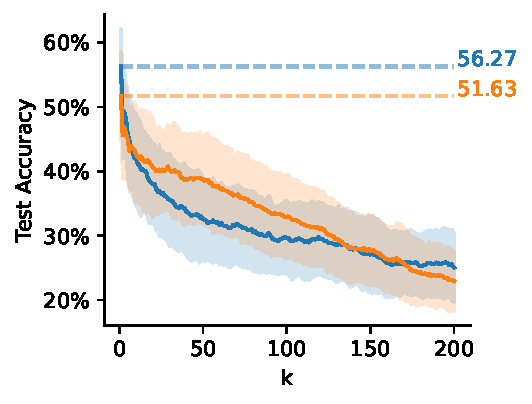
\includegraphics[width=\textwidth]{Figures/knn_ENZYMES.pdf}
		\vspace*{-4ex} 
		\caption{\textsc{Enzymes}}
	\end{subfigure}
	\hfill
	\begin{subfigure}[b]{0.3\textwidth}
		\centering
		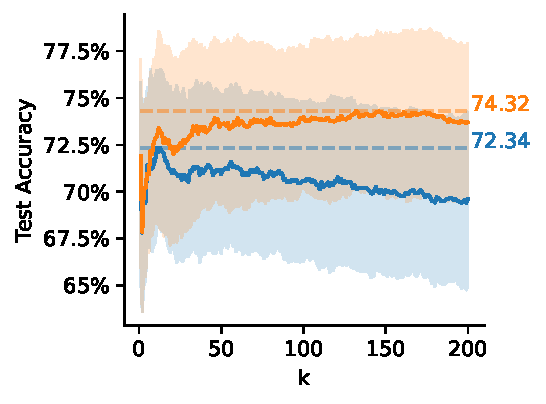
\includegraphics[width=\textwidth]{Figures/knn_IMDB-BINARY.pdf}
		\vspace*{-4ex} 
		\caption{\textsc{Imdb-Binary}}
	\end{subfigure}
	\hfill
	\begin{subfigure}[b]{0.3\textwidth}
		\centering
		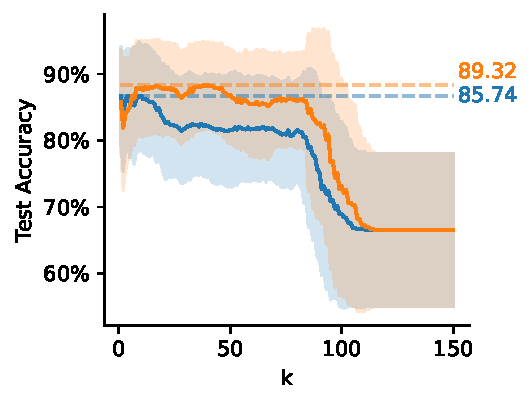
\includegraphics[width=\textwidth]{Figures/knn_MUTAG.pdf}
		\vspace*{-4ex} 
		\caption{\textsc{Mutag}}
	\end{subfigure}
	\par\bigskip
	\begin{subfigure}[b]{0.3\textwidth}
		\centering
		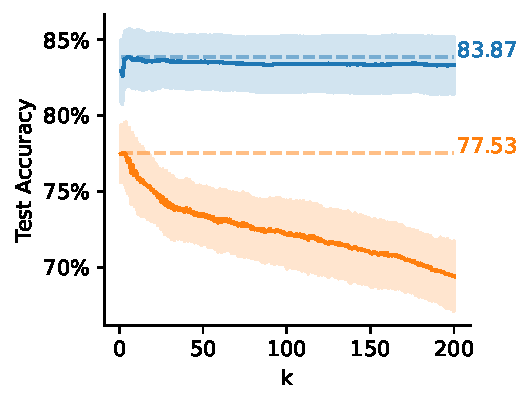
\includegraphics[width=\textwidth]{Figures/knn_NCI1.pdf}
		\vspace*{-4ex} 
		\caption{\textsc{Nci1}}
	\end{subfigure}
	\hfill
	\begin{subfigure}[b]{0.3\textwidth}
		\centering
		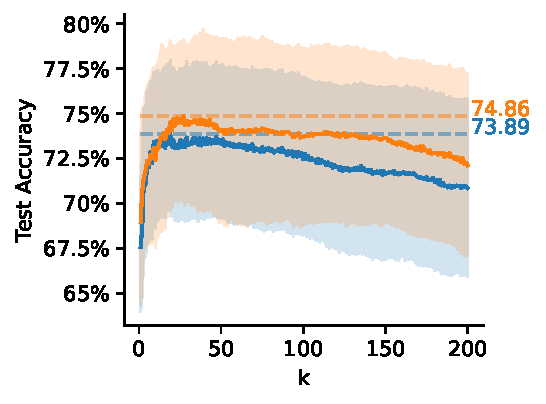
\includegraphics[width=\textwidth]{Figures/knn_PROTEINS.pdf}
		\vspace*{-4ex} 
		\caption{\textsc{Proteins}}
	\end{subfigure}
	\hfill
	\begin{subfigure}[b]{0.3\textwidth}
		\centering
		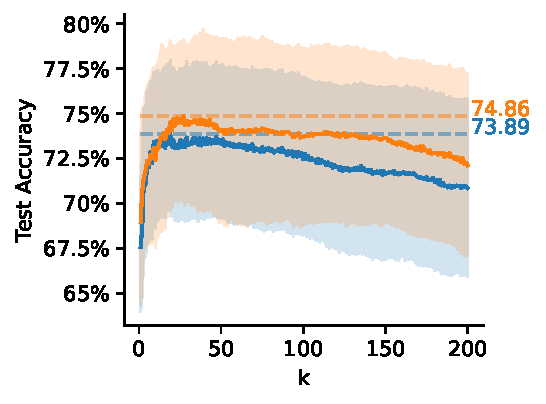
\includegraphics[width=\textwidth]{Figures/knn_PROTEINS}
		\vspace*{-4ex} 
		\caption{\textsc{Reddit-Binary}- MISSING}
	\end{subfigure}
	\centering
	\begin{subfigure}[b]{0.3\textwidth}
		\centering
		
\includegraphics[width=\textwidth]{Figures/train_test_diff_legend.pdf}
		\vspace*{-4ex} 
	\end{subfigure}
	\caption{Average classification accuracy achieved on each dataset by replacing the multilayer perceptron of the best-performing \wlnn and \gnn model with a classifier based on the $k$-nearest neighbors algorithm. We tested for different values of $k$.}
\end{figure}

\begin{figure}[H]
	\begin{subfigure}[b]{0.49\textwidth}
		\centering
		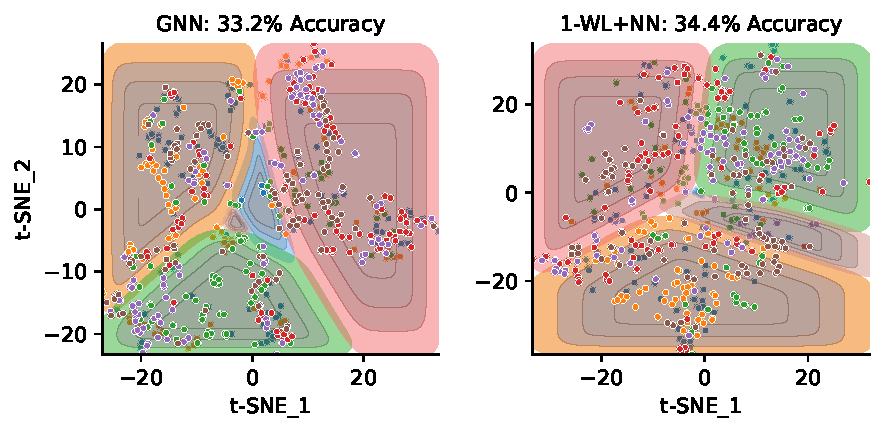
\includegraphics[width=\textwidth]{Figures/tsne_svm_lin_ENZYMES.pdf}
		\vspace*{-4ex} 
		\caption{\textsc{Enzymes}}
	\end{subfigure}
	\hfill
	\begin{subfigure}[b]{0.49\textwidth}
		\centering
		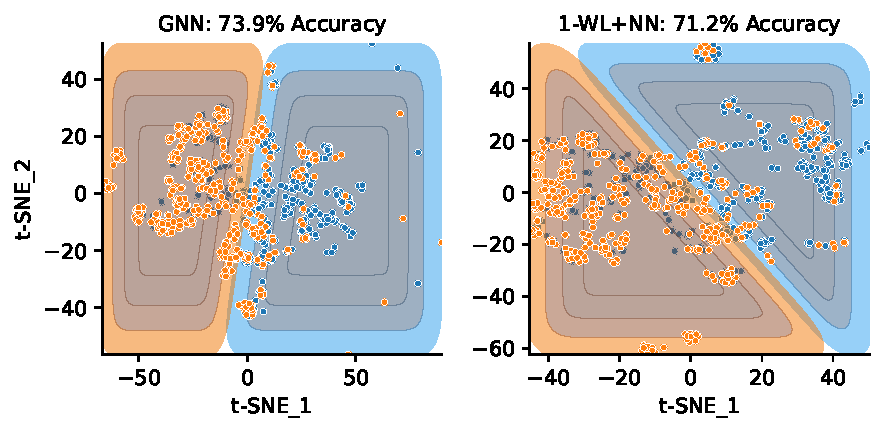
\includegraphics[width=\textwidth]{Figures/tsne_svm_lin_IMDB.pdf}
		\vspace*{-4ex} 
		\caption{\textsc{Imdb-Binary}}
	\end{subfigure}
	\par\bigskip
	\begin{subfigure}[b]{0.49\textwidth}
		\centering
		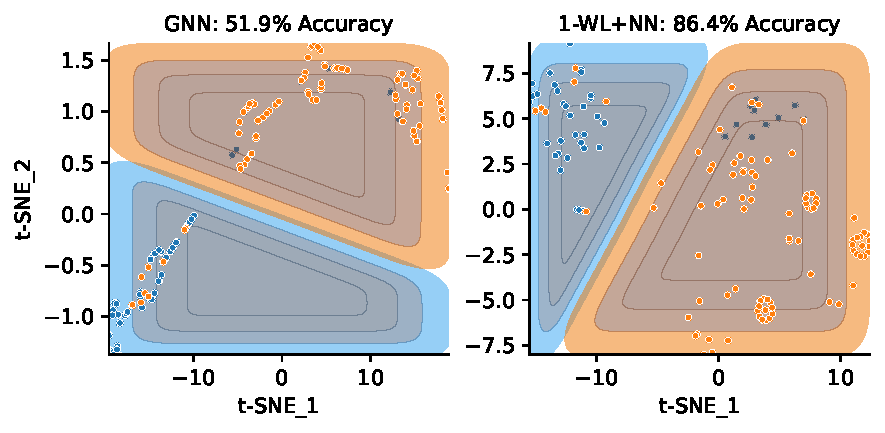
\includegraphics[width=\textwidth]{Figures/tsne_svm_lin_MUTAG.pdf}
		\vspace*{-4ex} 
		\caption{\textsc{Mutag}}
	\end{subfigure}
	\hfill
	\begin{subfigure}[b]{0.49\textwidth}
		\centering
		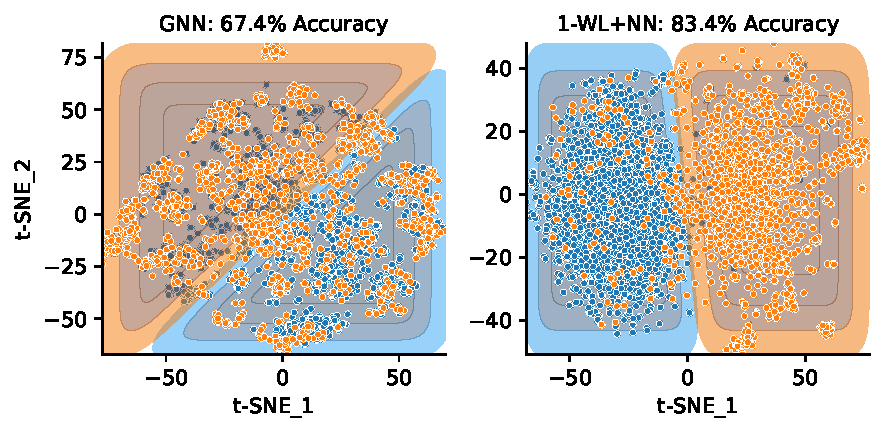
\includegraphics[width=\textwidth]{Figures/tsne_svm_lin_NCI1.pdf}
		\vspace*{-4ex} 
		\caption{\textsc{Nci1}}
	\end{subfigure}
	\par\bigskip
	\begin{subfigure}[b]{0.49\textwidth}
		\centering
		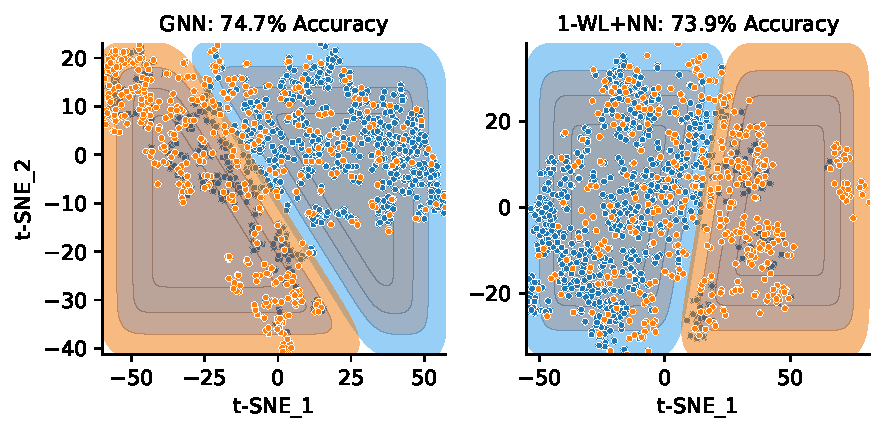
\includegraphics[width=\textwidth]{Figures/tsne_svm_lin_PROTEINS.pdf}
		\vspace*{-4ex} 
		\caption{\textsc{Proteins}}
	\end{subfigure}
	\hfill
	\begin{subfigure}[b]{0.49\textwidth}
		\centering
		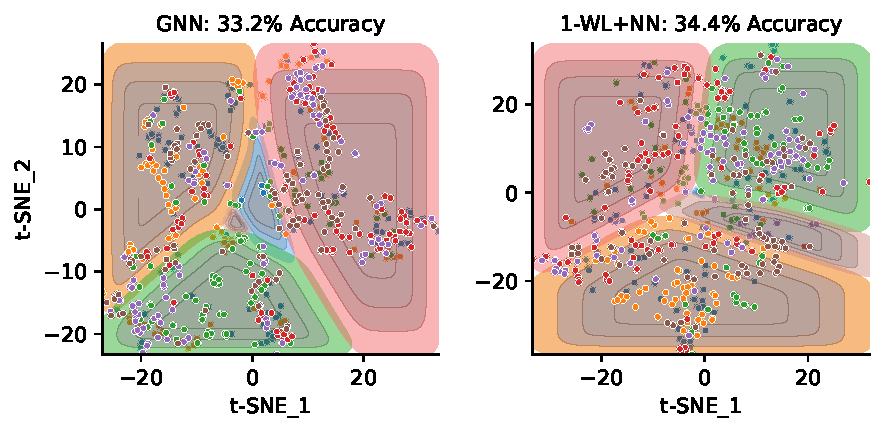
\includegraphics[width=\textwidth]{Figures/tsne_svm_lin_ENZYMES.pdf}
		\vspace*{-4ex} 
		\caption{\textsc{Reddit-Binary}- MISSING!}
	\end{subfigure}
	\caption{Visualization of the decision boundary of each Support Vector Machine with a linear kernel using t-SNE.}
\end{figure}

\begin{figure}[H]
	\centering
	\begin{subfigure}[b]{0.49\textwidth}
		\centering
		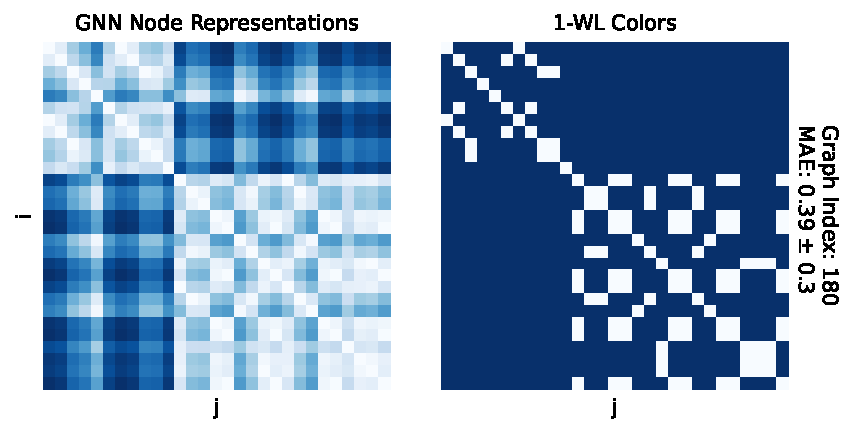
\includegraphics[width=\textwidth]{Figures/heatmaps_ENZYMES_single.pdf}
		\vspace*{-5ex} 
        \caption{\textsc{Enzymes}}
	\end{subfigure}
	\hfill
	\begin{subfigure}[b]{0.49\textwidth}
		\centering
		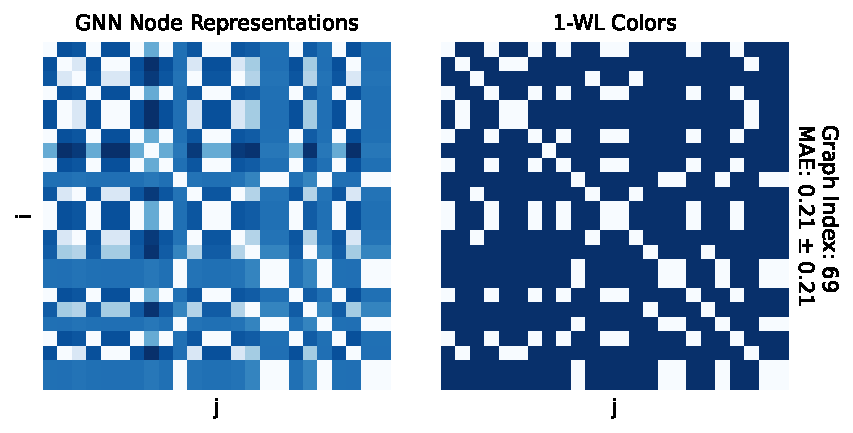
\includegraphics[width=\textwidth]{Figures/heatmaps_IMDB-BINARY_single.pdf}
		\vspace*{-5ex} 
        \caption{\textsc{Imdb-Binary}}
	\end{subfigure}
	\par\bigskip
	\begin{subfigure}[b]{0.49\textwidth}
		\centering
		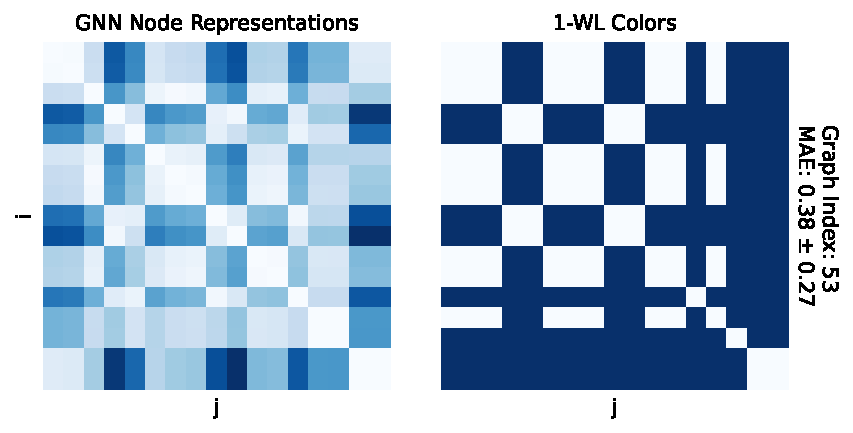
\includegraphics[width=\textwidth]{Figures/heatmaps_MUTAG_single.pdf}
		\vspace*{-5ex} 
        \caption{\textsc{Mutag}}
	\end{subfigure}
	\hfill
	\begin{subfigure}[b]{0.49\textwidth}
		\centering
		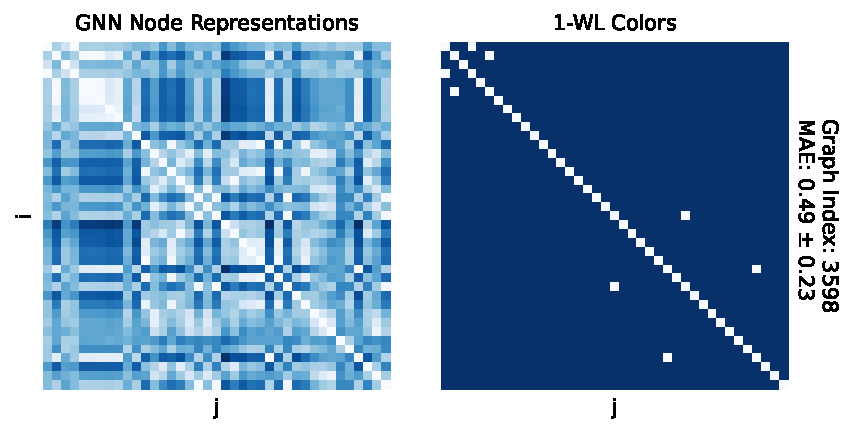
\includegraphics[width=\textwidth]{Figures/heatmaps_NCI1_single.pdf}
		\vspace*{-5ex} 
        \caption{\textsc{Nci1}}
	\end{subfigure}
	\par\bigskip
	\begin{subfigure}[b]{0.49\textwidth}
		\centering
		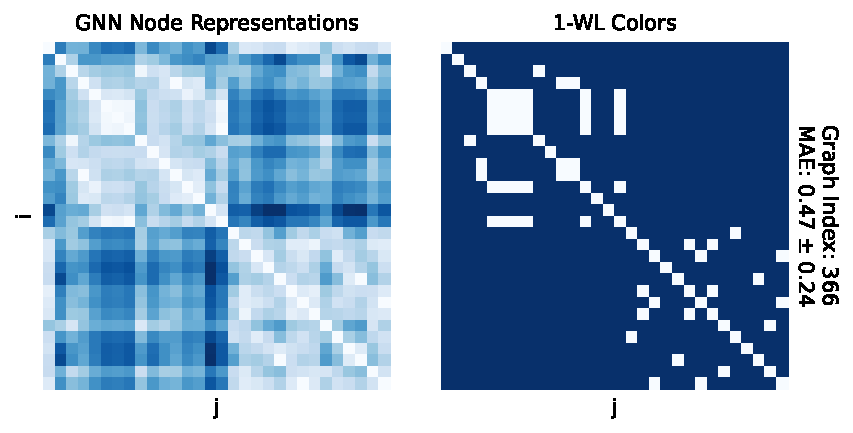
\includegraphics[width=\textwidth]{Figures/heatmaps_PROTEINS_single.pdf}
		\vspace*{-5ex} 
        \caption{\textsc{Proteins}}
	\end{subfigure}
	\hfill
	\begin{subfigure}[b]{0.49\textwidth}
		\centering
		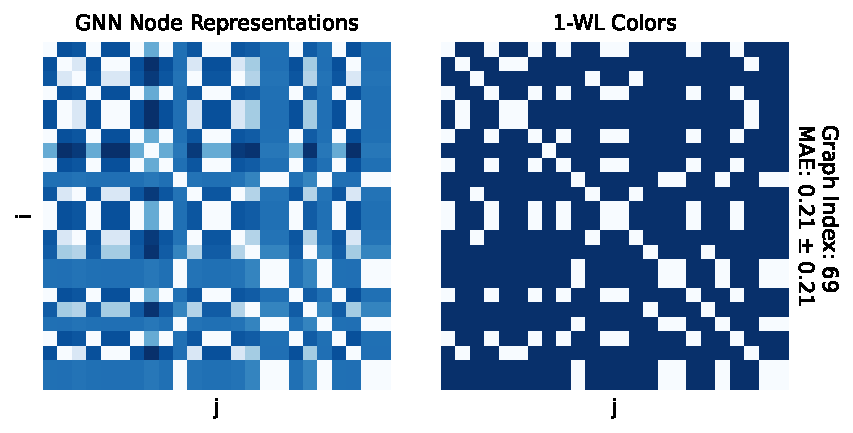
\includegraphics[width=\textwidth]{Figures/heatmaps_IMDB-BINARY_single.pdf}
		\vspace*{-5ex}
        \caption{\textsc{Reddit-Binary}-MISSING}
	\end{subfigure}
	\par\bigskip
	\begin{subfigure}[b]{0.6\textwidth}
		\centering
		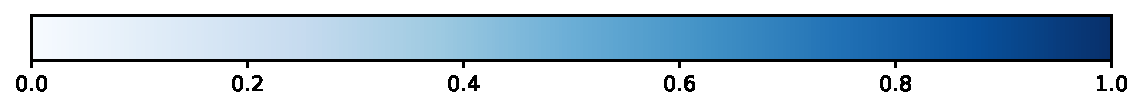
\includegraphics[width=\textwidth]{Figures/colorbar.pdf}
	\end{subfigure}
	\caption{Visualizing the performance of the best-performing \gnn models of each dataset in approximating node colors computed by the \wl algorithm. Here we randomly sampled a single graph for each dataset and visualized the approximation performance. For each calculation of the \wl colors, we utilized the number of iterations of the \wl algorithm to be the same as the best-performing \wlnn model of each dataset. Specifically, this was 1 for all datasets except for \textsc{Nci1}, where it was 3.}
\end{figure}

\begin{table}[H]
    \resizebox{.975\textwidth}{!}{ 	\renewcommand{\arraystretch}{1.05}
		\begin{tabular}{@{}c <{\enspace}@{}lcccccc@{}}	\toprule
			& \multirow{2}{*}{\vspace*{4pt}\textbf{Property}}&\multicolumn{6}{c}{\textbf{Dataset}}\\\cmidrule{3-8}
			& & {\textsc{Enzymes}}         &  {\textsc{Imdb-Binary}}      & {\textsc{Mutag}}           & {\textsc{NCI1}}       & {\textsc{Proteins}}           & 
			{\textsc{Reddit-Binary}}
			\\
			\toprule
			\multirow{1}{*}{}
			& MAE & 0.49 \scriptsize $\pm 0.3$ & 0.14 \scriptsize $\pm 0.15$ & 0.42 \scriptsize $\pm 0.29$
			& 0.42 \scriptsize $\pm 0.22$ & 0.49 \scriptsize $\pm 0.26$
			\\
			& Number of \wl colors & 230 & 64 & 32 & 27252 & 296 &
			\\
			\bottomrule
		\end{tabular}}
		\caption{MAE of the approximation performance of the best-perfoming \gnn in relation to the number of unique \wl colors for each dataset. In particular, in comparison to the colors computed by the \wl alogrithm with a single iteration.}
        \label{tab:my_label4}     
\end{table}

\begin{table}[H]
    \resizebox{.975\textwidth}{!}{ 	\renewcommand{\arraystretch}{1.05}
		\begin{tabular}{@{}c <{\enspace}@{}lcccccc@{}}	\toprule
			& \multirow{2}{*}{\vspace*{4pt}\textbf{Epsilon}}&\multicolumn{6}{c}{\textbf{Dataset}}\\\cmidrule{3-8}
			& & {\textsc{Enzymes}}         &  {\textsc{Imdb-Binary}}      & {\textsc{Mutag}}           & {\textsc{NCI1}}       & {\textsc{Proteins}}           & 
			{\textsc{Reddit-Binary}}
			\\
			\toprule
			\multirow{4}{*}{\rotatebox{90}{F1-Score}}
			& $\epsilon = 0.001$ & 52.55 & 60.97 & 62.01 &
			\\
			& $\epsilon = 0.01$ & 54.63 & 60.97 & 62.01 &
			\\
			& $\epsilon = 0.05$ & 62.33 & 71.68 & 62.01 & 
			\\
			& $\epsilon = 0.1$ & 70.45 & 78.66 & 62.01 &
			\\
			\cmidrule{2-8}
			& Number of \wl colors & 230 & 64 & 32 & 27252 & 296 &
			\\
			\bottomrule
		\end{tabular}}
		\caption{MAE of the approximation performance of the best-perfoming \gnn in relation to the number of unique \wl colors for each dataset. In particular, in comparison to the colors computed by the \wl alogrithm with a single iteration.}
        \label{tab:my_label4}     
\end{table}

\begin{figure}[H]
	\begin{subfigure}[b]{0.3\textwidth}
		\centering
		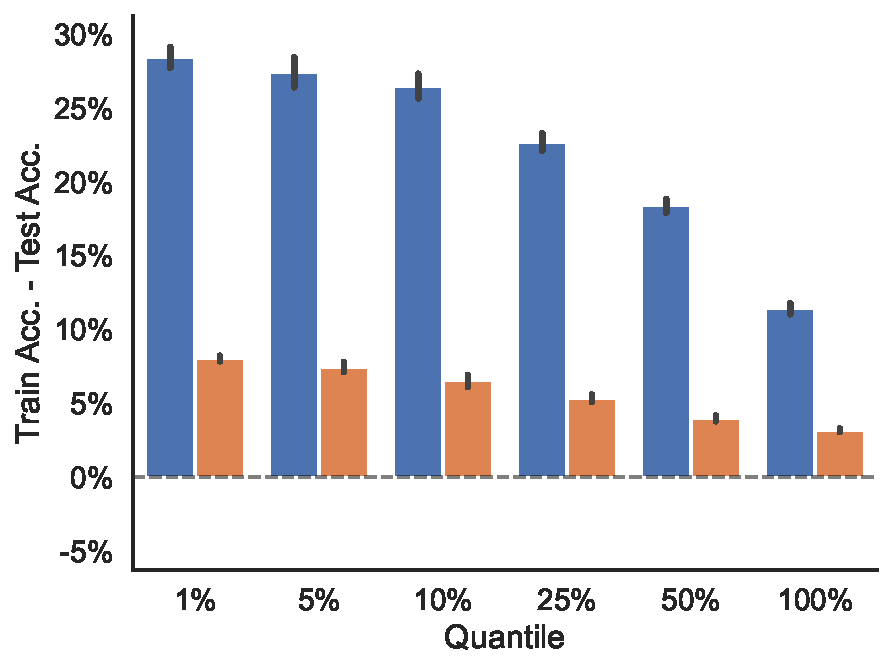
\includegraphics[width=\textwidth]{Figures/train_test_diff_ENZYMES.pdf}
		\vspace*{-4ex} 
		\caption{\textsc{Enzymes}}
	\end{subfigure}
	\hfill
	\begin{subfigure}[b]{0.3\textwidth}
		\centering
		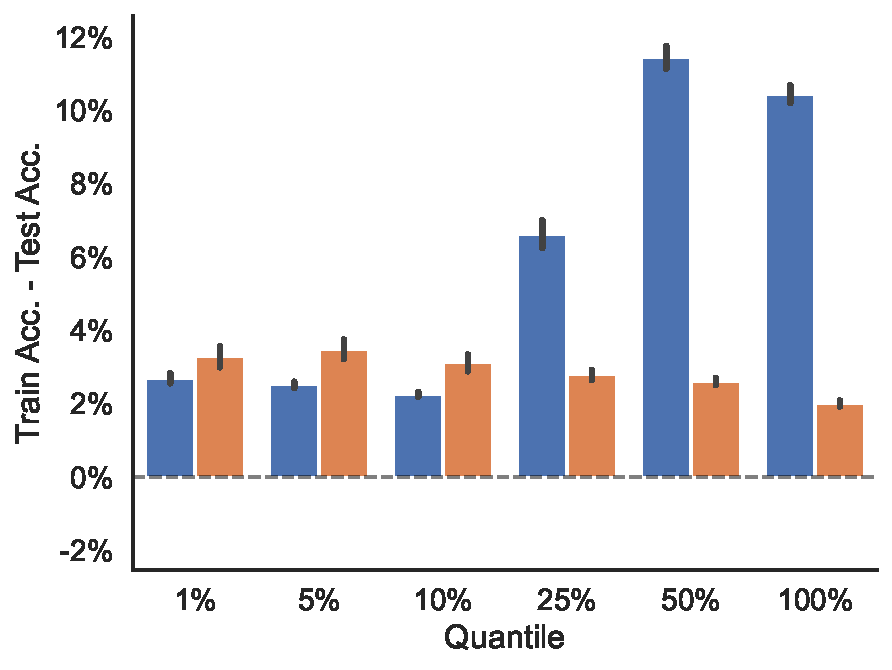
\includegraphics[width=\textwidth]{Figures/train_test_diff_IMDB-BINARY.pdf}
		\vspace*{-4ex} 
		\caption{\textsc{Imdb-Binary}}
	\end{subfigure}
	\hfill
	\begin{subfigure}[b]{0.3\textwidth}
		\centering
		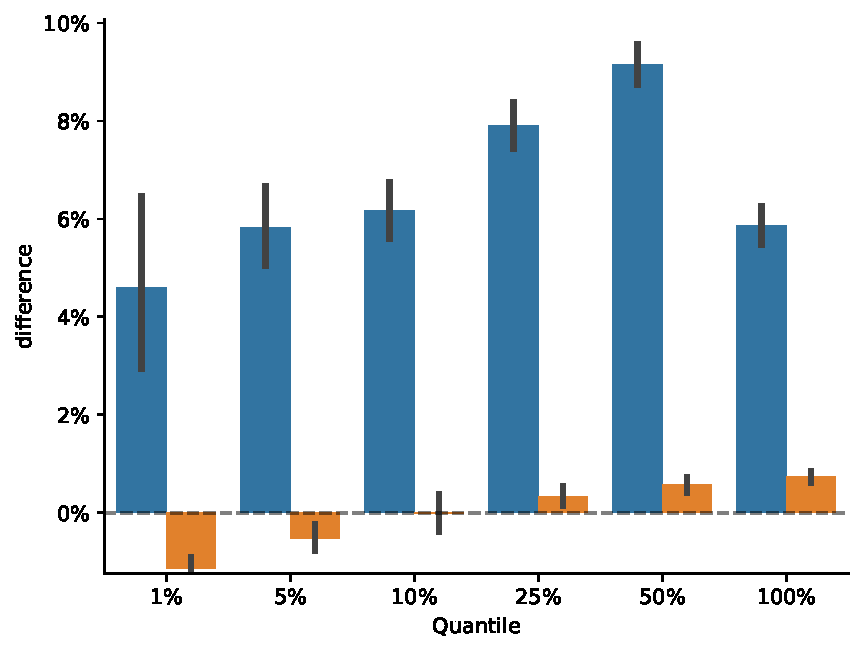
\includegraphics[width=\textwidth]{Figures/train_test_diff_MUTAG.pdf}
		\vspace*{-4ex} 
		\caption{\textsc{Mutag}}
	\end{subfigure}
	\par\bigskip
	\begin{subfigure}[b]{0.3\textwidth}
		\centering
		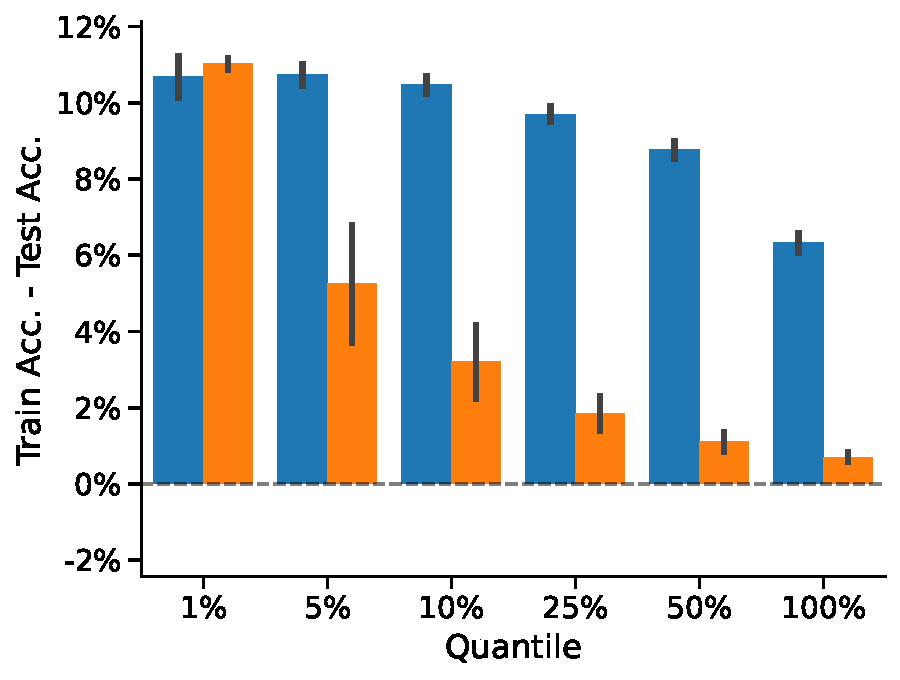
\includegraphics[width=\textwidth]{Figures/train_test_diff_NCI1.pdf}
		\vspace*{-4ex} 
		\caption{\textsc{Nci1}}
	\end{subfigure}
	\hfill
	\begin{subfigure}[b]{0.3\textwidth}
		\centering
		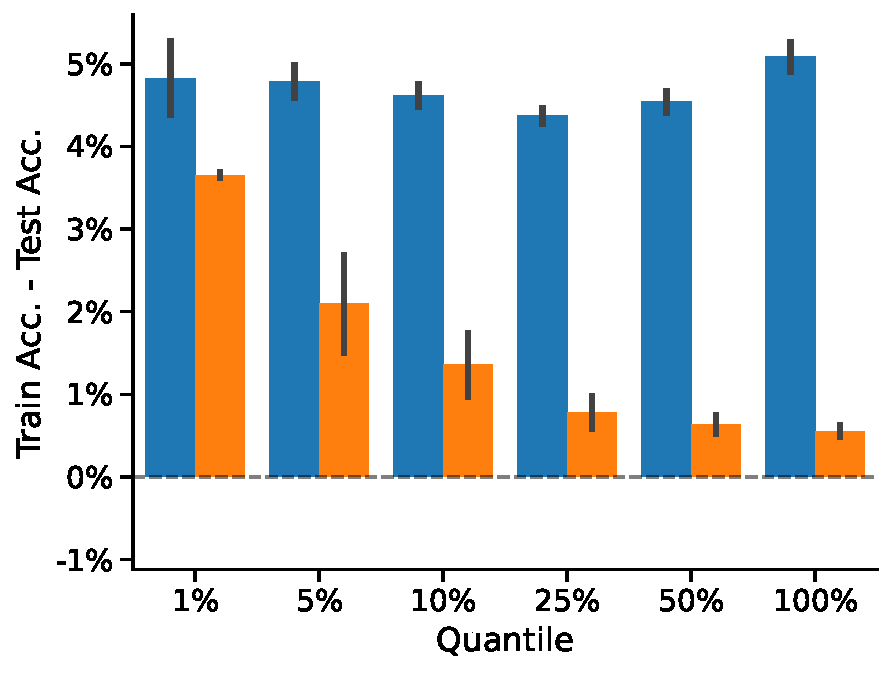
\includegraphics[width=\textwidth]{Figures/train_test_diff_PROTEINS.pdf}
		\vspace*{-4ex} 
		\caption{\textsc{Proteins}}
	\end{subfigure}
	\hfill
	\begin{subfigure}[b]{0.3\textwidth}
		\centering
		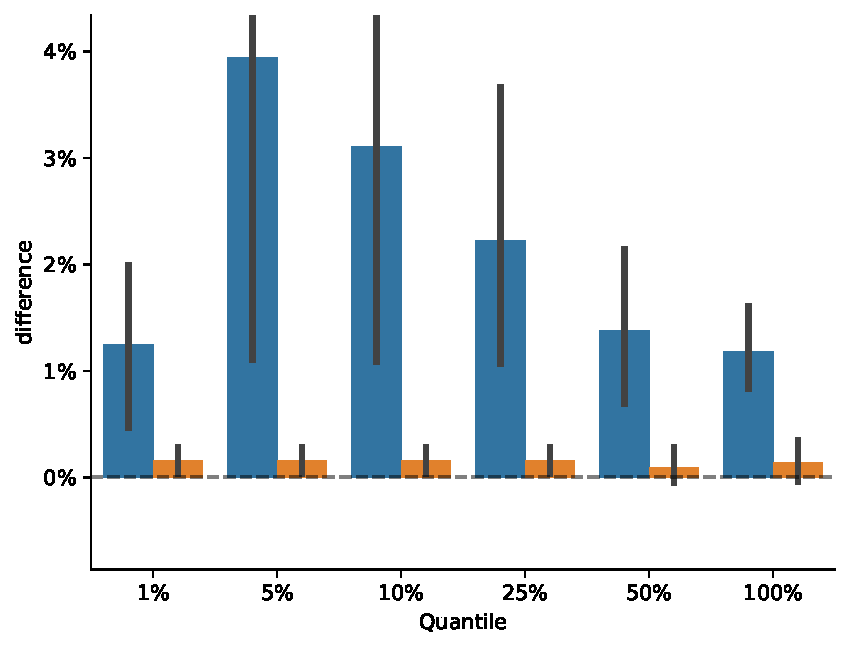
\includegraphics[width=\textwidth]{Figures/train_test_diff_REDDIT-BINARY.pdf}
		\vspace*{-4ex} 
		\caption{\textsc{Reddit-Binary}}
	\end{subfigure}
	\centering
	\begin{subfigure}[b]{0.3\textwidth}
		\centering
		
\includegraphics[width=\textwidth]{Figures/train_test_diff_legend.pdf}
		\vspace*{-4ex} 
	\end{subfigure}
	\caption{Mean absolute difference of the classification accuracies of the training and testing set of each dataset. In detail, we compared the different quantiles of each performance.}
\end{figure}

\chapter{These / Narrativ}
\begin{enumerate}
	\item \wlnn funktioniert nur sehr gut auf kleinen datasets:
	\begin{itemize}
		\item  Je größer das Dataset desto größer wird die 1-WL-Color ``Vielfalt'', schwierig für das MLP des \wlnn noch die richtigen Information rauszuziehen. -> These würde ich gerne noch überprüfen: Gibt es ein Classification Dataset das groß und gut ist? OGBG-Molhiv? MalNet Tiny?
		\item Dagegenspricht aber das die performance von NCI1 deutlich besser ist von \wlnn.
		\item Theorie warum \wlnn aktuell fast immer besser war, ist dass \wlnn viel weniger Parameter optimieren muss bei gleicher im Vergleich zu GNNs -> Optimum ist schneller gefunden!
		\item \gnn generalisieren besser im Sinne, dass sie unabhängig von der größe des Datasets sind. Alchemy zeigt das ganz gut!
		\item Difference in Training and Test Accuracy zeigt auch das die \wlnn Modelle stark overfitten -> Tendenz dazu dass mit größeren Datasets, generalisieren schwieriger wird.
		\item Performance von den \wlnn Modellen ohne Embedding (Look-Up-Table) ist auch nur auf kleinen Datasets gut. Je größer das Dataset desto größer ist die Differenz zwischen beiden Modell Konfigurationen.
	\end{itemize}
	\item GNNs approximiert \wl Farben:
	\begin{itemize}
		\item Aprroximation ist vorhanden und ist nicht so schlecht: Error ist zwar so circa bei 50\% dafür ist die std aber auch sehr hoch (circa 25\%).
		\item Vorallem approximierung von \wl mit nur einer Iteration (Node Degree!)
		\item Performance von den GNNs mit Node-degree initialiserung sind bis jetzt immer besser gewesen (IMDB-Binary \& Reddit-Binary)
	\end{itemize}
	\item GNNs und \wlnn erlernen graph representation die gut clustern:
	\begin{enumerate}
		\item Sehr gute lineare Separierbarkeit bei allen Datsets (Ausnahme ist Mutag wegen Bug!)
		\item k-NN clustering hoch für kleine k's bei beiden Modellen. Sehr ähnliche Accuracy Kurven!
		\item (t-SNE plots zeigen auch, dass clustering vorhanden ist.)
	\end{enumerate}
\end{enumerate}

		
F1  metric oder ROC (watch out unbalanced dataset)

-> intuition: gnn smoothen! (noise reduction)-> \gnn optimalere funktionen
Setup: de-noising notwendig, CSWM Problem konzipieren -> erst de-noising befor gute prediction
